%
\section{Findings}
%
Due to the subjective nature of estimating the overall quality of our video summaries we test our results on a panel of test users. We use various methods to generate the summaries and present them to the panel for review.
%
\subsection{Test Environment}
%
Our test environment is a website showing a collection of generated videos, hosted on YouTube. Visitors are shown one video at a time, and are presented with a questionnaire after the video is done playing.
%
\subsubsection{Questionnaire}\label{sec:questionnaire}
%
The questionnaire for each video consists of four statements to which the user can \textit{disagree}, \textit{somewhat disagree}, \textit{somewhat agree}, \textit{agree} or declare that she \textit{does not know}. In an attempt to discourage the user from selecting the latter option it is shown last. Based on feedback from an initial, single-user test run we also added and introduction page that explains the purpose of the test and shows the available statements and options. The description is also present throughout the test. Part of the website is shown in Figure \ref{fig:questdump}.\\
%
The four statements shown after a video is:
%
\begin{itemize}
\item The individual video clips are interesting
\item The video is well edited
\item The length of the individual video clips are fitting
\item The length of the entire video is fitting
\end{itemize}
%
The first statement investigates the quality of our choice of labels, and to some degree also the quality of our classifiers. The second statement investigates how well we are able to combine segments (in other words the quality of our recipe, ie. the order and context of the ingredients). The third statement investigates the general attitude towards clip-length, which is chosen somewhat at random within boundaries determined by the recipe. The fourth statement investigates the general attitude towards the total length of a video-summary. We also added an optional note to each questionnaire in case a user wanted to ellaborate on her answer(s).
%
\begin{figure}
     \centering
     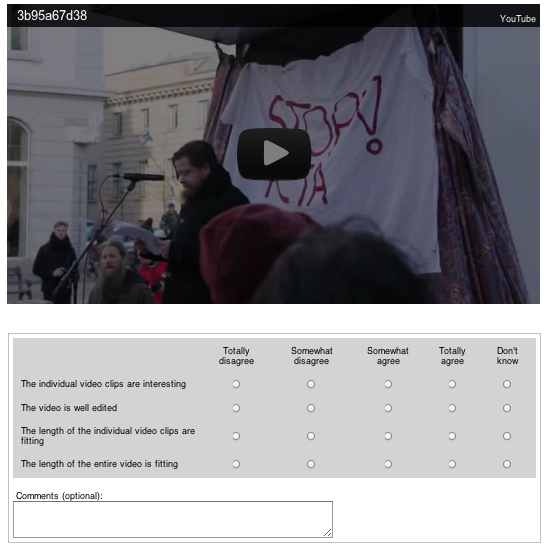
\includegraphics[width=1.0\textwidth]{img/quest_dump.png}
     \caption{Example of questionnaire on the test-site}\label{fig:questdump}
\end{figure}
%
\subsubsection{Setup}
%
Our test environment runs on \textit{Google App Engine} and consist of a minimalistic website. To discern interuptive elements player-controls are hidden in the embedded YouTube-player (the user can still pause the video). The questionnaire is not shown before the end of the video not to disctract the actual viewing. The video title appears briefly in the top of the player is a randomly generated non-descript title.\\
Each user session is tracked using a randomly generated identifier. We do not make any attempt to track users across different sessions and we are unable to track a returning test-user, but it does give us a rough measure of how many different test-users we have, how many questionnaires they answered on average.\\
To increase the availability of our test environment everything is localised into danish and english. The resulting locale is recorded along with each result, in case the specific translations have an effect on our results. All text in the test can be seen in figure \ref{fig:website}, in both languages.\\
The test is designed so that the test user can see as few or as many videos as she wants. A circular queue of videos is shared between all users, meaning that a new user will start at the video following the one that was last rated. Answers are stored after each succesful rating.\\
The test users concist of friends and relatives contacted through facebook. In order to help spread the test to more people we also placed a Facebook Like-button and a Twitter button discretely in the bottom of the questionnaires.\\\\
%
The test-site can be found at: http://thesis.fmitcar.appspot.com/thesis/start/ and a screendump of this is shown in Figure \ref{fig:website}
%
\begin{figure}
     \centering
     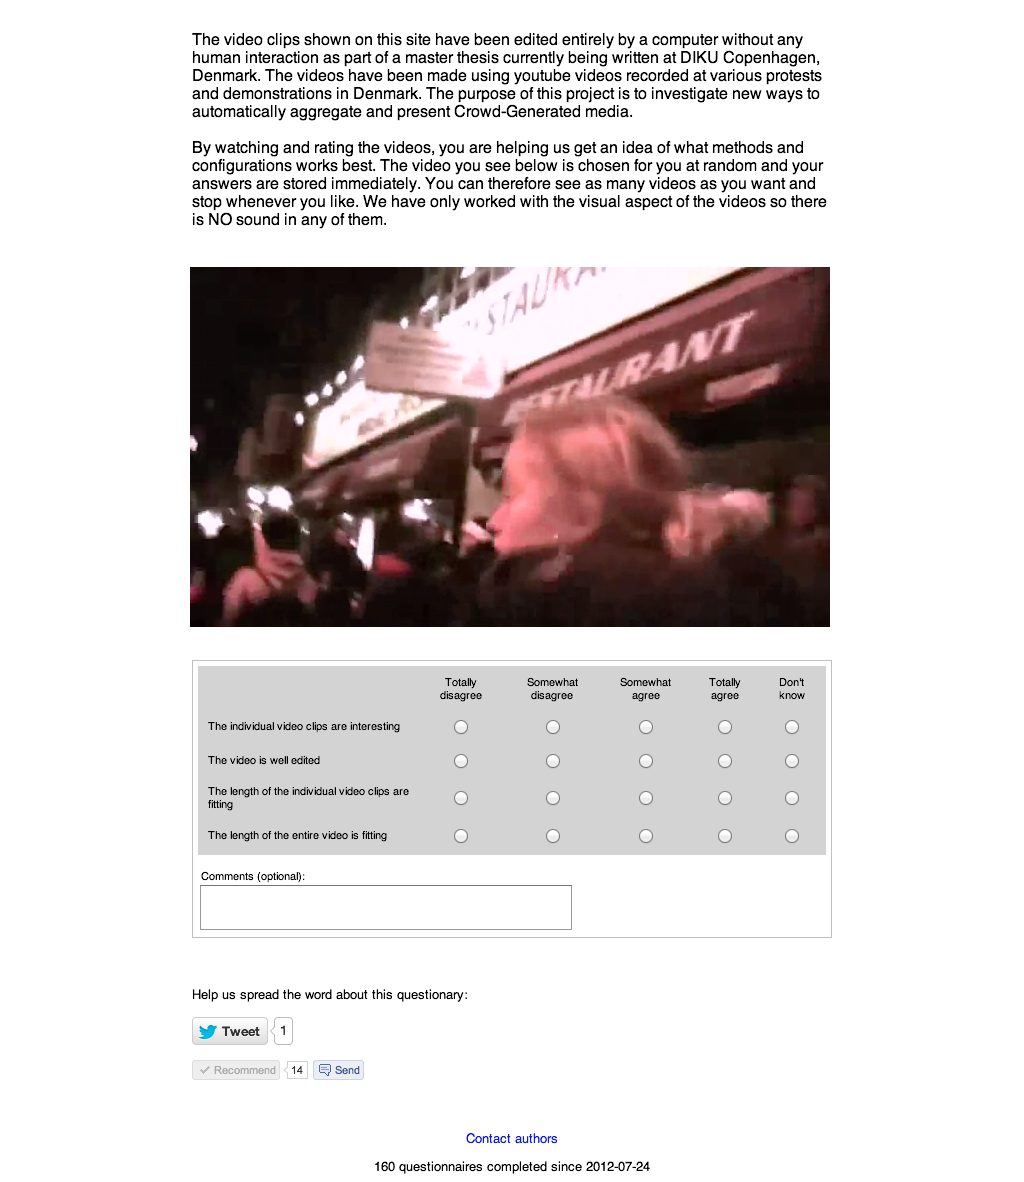
\includegraphics[width=1.0\textwidth]{img/website.png}
     \caption{Example of a page in the test-site}\label{fig:website}
\end{figure}
%
\subsection{Test videos}
%
We investigate several aspects of the video summary aggregation. Most importantly we investigate how our automatically generated video summaries compare to human edited ones, and how both these groups compare to randomly generated video summaries.\\
We generate the videos from all the labelled videos. Each video only uses footage from the event it is summarising.
%
\subsubsection{Random}
%
\textit{Random} video summaries are generated without any use of labels. They consist of 6 videoclips selected randomly from the footage for a particular event. Each clip has a random length between 2 and 10 seconds. Only one clip is selected from each video, in order to avoid repeating or overlapping footage, which would be a dead giveaway. These video summaries are thought of as a baseline - we expect them to perform poorly.
%
\subsubsection{Random label}
%
These video summaries are slightly \textit{less} random. Instead of selecting video clips randomly from the footage, we instead generate a random recipe and create a video summary from it. This is done by generating a sequence of 5 \textit{ingredients} (described in section \ref{sec:recipe}), each containing a random set of 1 to 3 \textit{requested labels}. The minimum length of a video clip, $min$, is randomly set to be between 2 and 9 seconds. The maximum length is randomly set to be between $min$ and $2 \cdot min$.\\
Because these video summaries are based on footage where labels were detected, we expect their content to be of higher quality than the videos described in the previous section.
%
\subsubsection{Designer}\label{sec:phase4designer}
%
The \textit{designer} video summaries are based on our own recipe. It tries to include segments of overview shots (segments classified positively by the \textit{overview} classifier), crowd shots (the \textit{in-crowd} classifier) and shots with persons in focus (\textit{person in focus} classifier). A minimum and maximum length for each segment is also defined. The ingredients are outlined below:
%
\begin{enumerate}
\item Overview shot, 3-5 seconds, no person in focus
\item Overview shot, 3-6 seconds, no person in focus
\item Crowd shot, 3-6 seconds, no person in focus
\item Crowd shot, 3-6 seconds, no person in focus
\item Person in focus shot, 4-8 seconds, not in a crowd
\item Person in focus shot, 4-8 seconds, not in a crowd
\item Overview shot, 3-5 seconds, no person in focus
\end{enumerate}
%
The list of ingredients also define the order of the segments in the final video summary. In order to compensate for the mediocre performance of the \textit{overview} classifier (detailed in section \ref{sec:peformanceforoverviewclassifier}), and the the extremely poor performance of the \textit{in-crowd} classifier (detailed in section \ref{sec:peformanceforincrowdclassifier}), we define \textit{person in focus} to be a forbidden label in all ingredients, where we do not specifically want such a segment. As described previously, a person in focus is the primary reason misclassifications in both classifiers.\\
\\
In an attempt to maintain contextual flow within the final video summary, we also require all daytime segments to preceed night-time segments. A segment breaking this rule is discarded and another is found. This only has an impact on the COP15 videos, as this dataset is the only which contain night-time footage.
%
\subsubsection{Human edited}
%
We used human edited video summaries as a control sample. These videos are taken from some of the orginal videos, which we found on YouTube and later split up. Therefore they contain the same footage as is available to the \textit{random-}, \textit{random label-}, and \textit{designer-} summarizers. This should ensure that they do not look too different. We expect these to perform as well as the designer recipies or better.
%
\subsubsection{Other aspects}\label{sec:otheraspects}
%
On top of comparing the quality of the different types of videos described above, we also investigate the result of using different $\alpha$ values to regulate the weighting between label- and timespan- fulfilment. Different values should affect both the length of the individual video clips, and the total length of the video summary. We experiment with $\alpha=0.25$ and $alpha=0.50$. Higher values gives to much priority to the timespan, which means that the content of the final video summary becomes to difficult to control.\\
Finally, we also want to know if the actual events in the footage has any influence of our results.\\\\
%
In total there are 21 videos summaries in the test. Their distribution is shown in figure \ref{tab:videosintest}.
%
\begin{table}\centering
    \begin{tabular}{|l|l|l|l|}
        \hline
        Method       & Event           & $\alpha$      & YouTube ID \\ \hline
        random       & ACTA Aarhus     & ~             & 5swFsRKsI7I \\ % 2806c14722
        random       & ACTA Copenhagen & ~             & XYHr6gZqkTs \\ % 48b62f11dc
        random       & COP 15          & ~             & hrxbQNTBqNQ \\ % dd7d1998f8
        random label & ACTA Aarhus     & 0.25          & pBw6UJa6-\_w \\ % 7babfd31c4
        random label & ACTA Aarhus     & 0.50          & 8sk2HWj4zhU \\ % 3b95a67d38
        random label & ACTA Copenhagen & 0.25          & G9YeDzzwyVQ \\ % 143a413f62
        random label & ACTA Copenhagen & 0.50          & a7k7gemEwsE \\ % 80a451d4c2
        random label & COP 15          & 0.25          & ho1CjPB02F8 \\ % 90fe6adcd2
        random label & COP 15          & 0.50          & 2C7Y5Shw5p8 \\ % d370ccc56c
        designer     & ACTA Aarhus     & 0.25          & BbS0GQLp4CQ \\ % a8d1de1e81
        designer     & ACTA Aarhus     & 0.50          & yrfnIujswX8 \\ % 98b1d02056
        designer     & ACTA Copenhagen & 0.25          & 75IHEvP7An4 \\ % 9891596ecf
        designer     & ACTA Copenhagen & 0.50          & E1v6\_GvB3j4 \\ % 913eef2ed2
        designer     & COP 15          & 0.25          & 48QPI1wz1QY \\ % bf7dc9f5ca
        designer     & COP 15          & 0.50          & j\_pkzYcJ8j0 \\ % 625838c2b1
        human edited & ACTA Copenhagen & ~             & MLzAuBHSiTU \\ 
        human edited & ACTA Copenhagen & ~             & ZFSYWB1BcxE \\ 
        human edited & ACTA Copenhagen & ~             & Mu7JJEHonGE \\ 
        human edited & ACTA Copenhagen & ~             & rEFkglQCcXg \\ 
        human edited & COP 15          & ~             & 7sao2\_7sKms \\ 
        human edited & COP 15          & ~             & HlOIeCzXSCI \\
        \hline
    \end{tabular}
\caption{Distribution of videos in the test}\label{tab:videosintest}
\end{table}
%
\subsection{Results}
%
We start by looking at an overview of the data we gathered, and then go into detail with the specific results.
%
\subsubsection{Feedback}
%
At the time of writing, our test has been online for around 4 weeks. In that time 160 videos have been observed and rated over 25 sessions.\\
The average number of answers per session is 6.4, with a median of 5.0. The shortest session contains 1 answer and the longest contain 25\\
In addition to the answers required for each video, we also received 11 notes from the test users as can be seen in table \ref{tab:notes}.\\
108 (67.5\%) are answers from the danish version of the test. 52 (32.5\%) is from the enlish version. Each videos in the test is rated 7 or 8 times.
%
\subsubsection{Histograms}\label{sec:histograms}
%
Histograms shows the distribution of data, and is a visual tool to aid in determining if data follows a specific probability distribution. There are 5 bins in the histograms, where each bin corresponds to a specific answer to our questionnaire. Each bin is thus, from left to right, Totally Disagree (TD), Somewhat Disagree (SD), Don't Know (DK), Somewhat Agree (SA), Totally Agree (TA). The answers are divided into groups based on how they where created, as described in section \ref{sec:otheraspects}.
%
\begin{figure}[!ht]
     \centering
     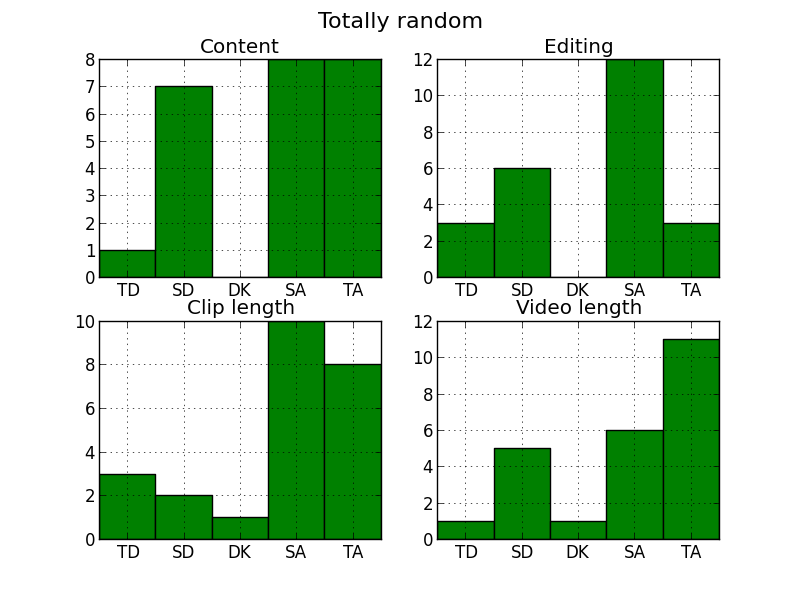
\includegraphics[width=0.7\textwidth]{img/totallyrandom_barplot.png}
     \caption{Histogram of answers to videos created using random segments}\label{fig:hist_random}
\end{figure}
%
\begin{figure}[!ht]
     \centering
     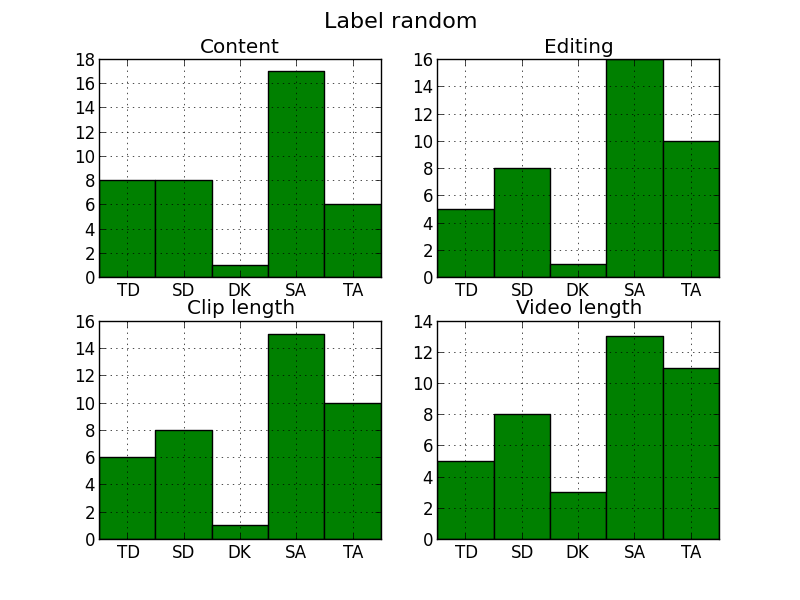
\includegraphics[width=0.7\textwidth]{img/labelrandom_barplot.png}
     \caption{Histogram of answers to videos created using the random label recipe}\label{fig:hist_labelrandom}
\end{figure}
%
\begin{figure}[!ht]
     \centering
     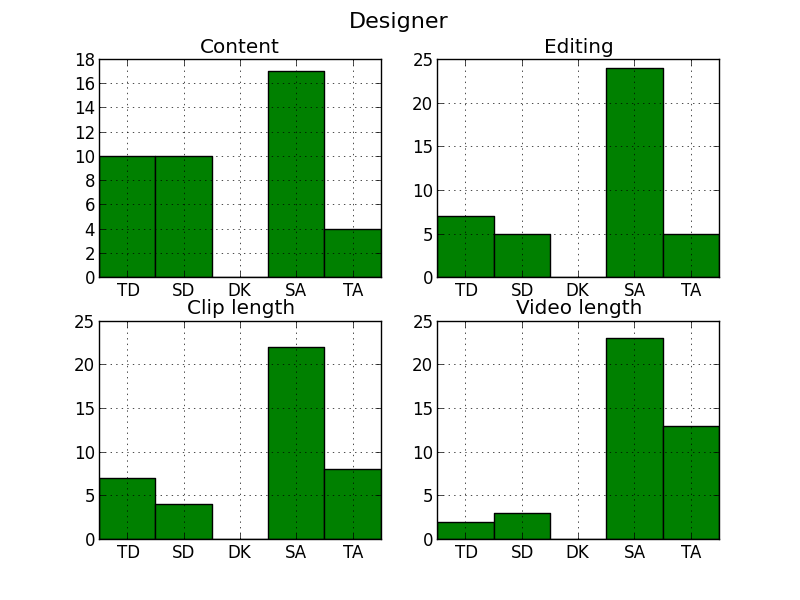
\includegraphics[width=0.7\textwidth]{img/designer_barplot.png}
     \caption{Histogram of answers to videos created using the designer method}\label{fig:hist_design}
\end{figure}
%
\begin{figure}[!ht]
     \centering
     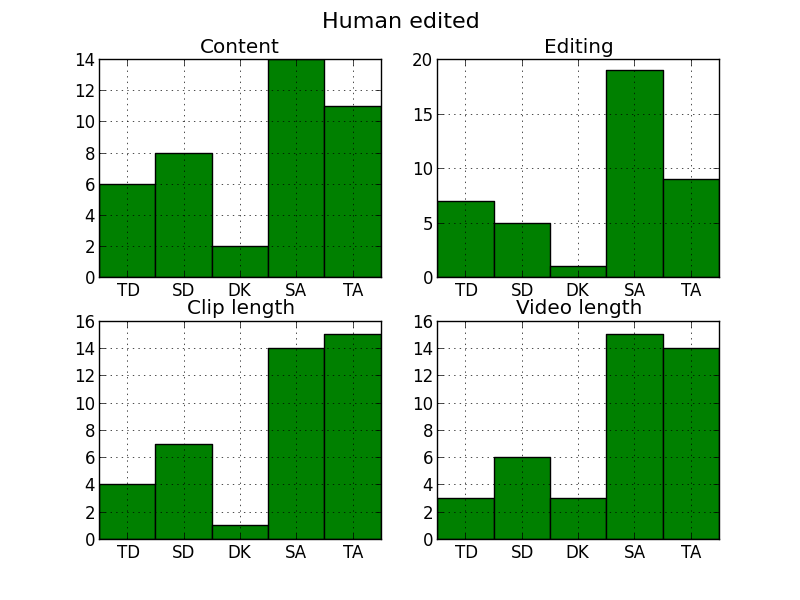
\includegraphics[width=0.7\textwidth]{img/humanedited_barplot.png}
     \caption{Histogram of answers to videos that are edited by a human}\label{fig:hist_human}
\end{figure}
%
\subsubsection{Friedman Test}\label{sec:friedman}
%
The Friedman rank sum test
% KIM: reference
 is a non-parametric statistical test, and is used to detect differences in methods in multiple tests. In our case we have multiple methods, datasets, and parameters, and each test participant can be viewed as a seperate test.\\
 We test against the null-hypotheses stated as follows: 
 %
 \begin{itemize}
 \item There is no significant measureable difference in the methods used to generate a video
 \item There is no significant measureable difference in the dataset used to generate a video
 \item There is no significant measureable difference in the $\alpha-$span parameter used to generate a video
 \end{itemize}
%
The histograms in section \ref{sec:histograms} shows us that the data does not follow any specific distribution, which forces us to deploy a non-parametric statistical test. The disadvantage of employing a non-parametric test is that it requires a larger sample size to draw conclusions with the same degree of confidence as a parametric test.\\
%
The values related to each answer are also not compareable (there is no clear numerical interpretation), ie. \textit{Totally Disagree} $(-2)$ is not twice as bad as \textit{Somewhat Disagree} $(-1)$, but \textit{Totally disagree} is ranked lower than \textit{Somewhat disagree}. The Friedman test ranks all answers, where answers with equal values receive the same rank, and then sums occurences of each rank.\\
%
Results of our Friedman test can be found in Tables \ref{tab:fried_alpha}, \ref{tab:fried_dataset}, and \ref{tab:fried_recip} where $\nu$ denotes degrees of freedom, and p-value is \textit{"the probability of obtaining a test statistic at least as extreme as the one that was actually observed, assuming that the null hypothesis is true."}\footnote{http://en.wikipedia.org/wiki/P-value}. A p-value less than $0.05$ is considered statistically significant.
% INPUT IS 3 TABLES
\begin{table}[ht]
	\begin{center}
	\caption{Friedman rank sum test for recipies}
	\label{tab:fried_recip}
		\begin{tabular}{lccc}
		\toprule
			 & v & p-value & $x^2$\\
			\midrule
			Content & $3$ & $0.3242$ & $3.4737$\\
			Editing & $3$ & $0.3260$ & $3.4602$\\
			Clip length & $3$ & $0.9597$ & $0.3016$\\
			Video length & $3$ & $0.3218$ & $3.4918$\\
			Total score & $3$ & $0.4882$ & $2.4292$\\
		\bottomrule
		\end{tabular}
	\end{center}
\end{table}
\begin{table}[ht]
	\begin{center}
	\caption{Friedman rank sum test for datasets}
	\label{tab:fried_dataset}
		\begin{tabular}{lccc}
		\toprule
			 & v & p-value & $x^2$\\
			\midrule
			Content & $2$ & $0.0773$ & $5.1193$\\
			Editing & $2$ & $0.5436$ & $1.2190$\\
			Clip length & $2$ & $0.0577$ & $5.7059$\\
			Video length & $2$ & $0.2030$ & $3.1887$\\
			Total score & $2$ & $0.1185$ & $4.2656$\\
		\bottomrule
		\end{tabular}
	\end{center}
\end{table}
\begin{table}[ht]
	\begin{center}
	\caption{Friedman rank sum test for $\alpha$-span}
	\label{tab:fried_alpha}
		\begin{tabular}{lccc}
		\toprule
			 & v & p-value & $x^2$\\
			\midrule
			Content & $1$ & $0.7055$ & $0.1429$\\
			Editing & $1$ & $1.0000$ & $0.0000$\\
			Clip length & $1$ & $0.4652$ & $0.5333$\\
			Video length & $1$ & $0.7055$ & $0.1429$\\
			Total score & $1$ & $0.5271$ & $0.4000$\\
		\bottomrule
		\end{tabular}
	\end{center}
\end{table}
%
\\
Table \ref{tab:fried_recip} shows the result from videos generated by the each method, Table \ref{tab:fried_dataset} shows the results from videos partitioned by which dataset a given video is generated from, and Table \ref{tab:fried_alpha} shows the effect of different $\alpha$-span values (described in section \ref{sec:recipe})
%
\subsubsection{Comments}\label{sec:comments}
%
Table \ref{tab:notes} show some of the comments we recieved on each video. We have omitted the specific video in question, but have shown the recipe the video was created with and also the dataset the video is based on. The comments are shown unedited in their original language.
%
\begin{table}[ht]
	\begin{center}
	\caption{Comments to videos in questionnaire}
	\label{tab:notes}
		\begin{tabular}{l l p{7.5cm}}
		\toprule
			dataset & recipe & note\\
			\midrule
			ACTA Aarhus & Random Label & "Stop ACTA" message is conveyed throughout the clip, which is nice.\\
			COP15 & Random & Lot's of action in the beginning, then slows down :)\\
			COP15 & Designer & Et klip af kajakroere virkede malplaceret. (Del Pin)\\
			ACTA Cph. & Human Edited & Virkede underligt at et klip var fast forward. (Del Pin)\\
			COP15 & Designer & Klip med politi (fra Jagtvej 69?) stod lidt ud.\\
			COP15 & Human Edited & Jeg synes det er sv\ae rt at besvare sp\o rgsm\aa lene i et tomrum. Fx vil noget typisk v\ae re interessant ej ikke i forhold til noget andet. (Del Pin)\\
			ACTA Cph. & Human Edited & Igen, skulle jeg forstille mig det var en teaser for en n\ae ste demonstration, et nyhedsindslag eller noget tredje? En videos l\ae ngde kan d\aa rligt i sig selv v\ae re passende. (Del Pin)\\
			ACTA Aarhus & Designer & Irriterende at nogle klip af samme motiv var i tydeligt d\aa rligere tilstand. (Del Pin)\\
			ACTA Cph. & Random Label & Nothing's happeningn for the first long time, then we see people who jump. Not enought action for me ;)\\
			ACTA Aarhus & Designer & De enkelte klip bliver un\ae gteligt mindre interessante, n\aa r jeg skal se p\aa  dem for 7. gang. (Del Pin)\\
		\bottomrule
		\end{tabular}
	\end{center}
\end{table}
%
\subsection{Analysis}
%
We generally receive positive feedback on the videos. Figure \ref{fig:hist_random} (random) and \ref{fig:hist_human} (human edited) shows that answers are unevenly distributed with a skew to the right, ie. test participants generally agrees with the statements. Figure \ref{fig:hist_labelrandom} (random label) shows that answers are somewhat evenly distributed, not counting the \textit{don't know} answer. Figure \ref{fig:hist_design} (designer) shows that answers are unevenly distributed with a skew to the right with the exception of the \textit{content} statement.\\
We are unable to reject the null hypothesis in almost all regards and conclude that the questionaires reveal no significant effect on the various methods of generating a video. This also means that there is no significant measureable difference between a human edited video and one that is generated at random.\\
%
There is also no significant measureable effect of choosing different $\alpha$-values when generating videos. This means that we are unable to discern if longer or shorter scenes in a video is desired.\\
%
There was also no significant measureable difference between the three datasets, except in content, which is no surprise as the datasets differ primarily on content as described in section \ref{sec:dataset}.\\
%
We have omitted analysis of the comments in Table \ref{tab:notes} and instead included them in the discussion section of this chapter.\\
%
\subsection{Discussion}
%
The histograms shows that test participants are generally in agreement with the statements proposed to them. This could be the result of their familiarity with the authors, as they may be inclined give positive answers, when in doubt.\\
The test revealed no significant measureable effect in any regard, and we believe that one of the causes is high quality raw material. We suspect that there would have been a noticeable difference if our dataset had contained a larger amount of video footage of questionable quality; both visual and contextual. This does however primarily account for the questionnaire statement regarding content, since the other statements are related to the actual editing of the footage.
%
\subsubsection{Risks and Limitations}
%
The lack of significantly measureable results can be a result of the questionnaire. The wording of each statement (and answer the thereto), as described in section \ref{sec:questionnaire}, may not give us the information we are looking for.\\
Based on feedback from users (both through the test and in person) we have come to understand that several things could have been done better. Several users complained over the lack of context in which they were watching the video. They claimed, rightfully, that it is difficult to determine whether clips were interresting or whether the length of a video is fitting, when they did not know what they were watching. The lack of sound only makes this more difficult. One suggestion for improvement, we received, was to preceed each statement with a written context describing what was being shown.\\
\\
A non-parametric statistical test usally requires a larger sample size, in order to be useful for drawing conclusions with the same degree of confidence as a parametric test, as mentioned in section \ref{sec:friedman}. We only received 7 to 8 answers for each video.\\
\\
The total number of videos for each type (random, designer, etc.) could also be a problem. We had to keep the number low in order to make sure that we received the number of answers for each video, we needed. As described above, even with just 21 one videos, we still did not receive enough answers.\\
\\
Our dataset itself is also a problem. We only use $\sim$ 90 minutes of footage for the final summary aggregation. Of this, only a part is actual raw footage. The rest is from pre-edited videos, which we later split up into individual scenes and use as raw footage (as described in section \ref{ph1:preeditedyoutube}). This is bound to increase the overall quality. This could be a reason why the \textit{random} and \textit{random label} videos, which are suppose to function as baselines in the test, still perform rather well.
%
\section{Summary}
%
We have described a way to automatically generate video summaries based on a defined \textit{recipe}. We have shown how the structure of this recipe can be used to compensate for some of the shortcomings of the various label classifiers we described in chapter \ref{chp:group_and_label}.\\
We have described a method for estimating how well a segment of footage fulfills a specific requirement, as defined by an ingredient in a recipe. This meassure of fulfillment can be used as an indicator for what segments to include in the final video.\\
We have compared this method with various control groups, both consisting of randomly generated-, but also of humanly edited- videos. This was done through an online survey were a group of test users observed the different videos and rated them on various aspects, such as content, length, and editing quality.\\
The results from this survey are inconclusive. The test users ability to differentiate between the various types of videos is not statistical significant. We have speculated on the various possible reasons for these findings and concluded that a lack of feedback, as well as the ambiguity in the phrased statements in the test, may be the cause.